The N-Queens puzzle is the problem of placing N chess queens on an NxN
chessboard so that no pair of two queens attack each
other~\cite{8queens}. The challenge of finding all the
distinct solutions to this problem is a good benchmark in designing
parallel algorithms.

The CLM solution considers the squares of the chess board as a graph
of nodes which exchange valid configurations with each
other. Initially every square in the first row of the board gets the
empty state.  Then, each square adds its own position to the state and
sends the state down, to the next row. Once a square receives new
configurations, it attempts to add its position to the
configurations. If valid, that configuration is then sent,
recursively, to the next row, until all rows are traversed. At the end
of the program, the squares at the bottom row will have all the valid
configurations.

Since computation goes from the top row to the bottom row, not all
placements of nodes to threads performane equally. This is especially
true because the bottom rows tend to perform the most work. The best
placement is then to split the board vertically so each thread gets
the same number of columns with axiom \texttt{set-cpu(A, vertical(X, Y)}, where
\texttt{X} and \texttt{Y} are the coordinates of the board. Our experiments show that, on a shared
memory system, it does not matter much if we start with a bad
placement since node stealing overcomes those issues by load balancing
dynamically.  However, the N Queens program incrementally builds and shares lists representing
valid board states that are transmitted from top to bottom.
In order to improve memory locality we should then manipulate board
states that share a significant number of elements because each board state
needs to be iterated before extended with a new position.
To accomplish this, we used coordination axioms \texttt{set-default-priority(A,
X)}, where \texttt{X} is the row number (0 is the top row) in order to
prioritize the evaluation of squares closer to the bottom of the board.

Experimental results are presented in Fig.~\ref{results:nqueens}.  We
first ran the coordinated program using dynamic partitioning (with
work stealing) and saw some performance improvements
(\textbf{Coordinated}). However, using dynamic partitioning is bad for
memory locality since threads will often steal nodes.  We then
added \texttt{set-static(A)} as a coordination axiom and saw
performance improvement (\textbf{Static}), especially when the board
columns are perfectly partitioned by the number of threads (in our
case 13 threads).

\begin{topfig}
   \begin{center}
      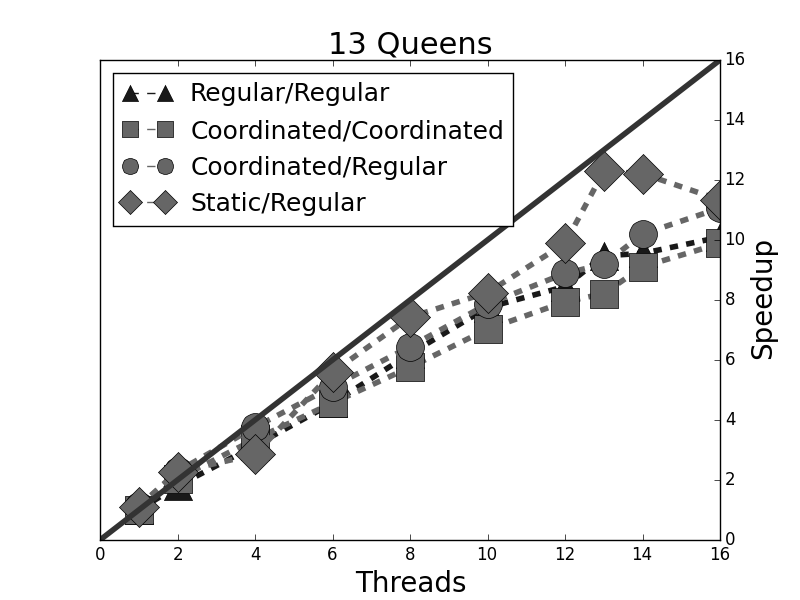
\includegraphics[width=5.5cm]{results/8queens-13.png}
   \end{center}
   \scap{results:nqueens}{Experimental results for the 13 Queens program.
   Coordination works best when 1 column is assigned to one thread and bottom
   rows have higher priority.}
\end{topfig}
